\documentclass[12pt,a4paper]{article}

\usepackage[a4paper, margin=2.5cm]{geometry}
\usepackage{graphicx}
\usepackage{booktabs}
\usepackage{caption}
\usepackage{subcaption}
\usepackage{float}
\usepackage{algorithm}
\usepackage{algpseudocode}
\usepackage[T1]{fontenc}
\usepackage[utf8]{inputenc}
\usepackage{hyperref}
\captionsetup{font=small,labelfont=bf,format=plain,justification=justified}
\renewcommand{\thefigure}{S\arabic{figure}}
\renewcommand{\thetable}{S\arabic{table}}

\begin{document}

\begin{center}
{\Large\bfseries Supplementary Material for QMOF-Rec}\\[0.5em]
{\normalsize Representative Candidate-Conditioned Interface Screenshots}
\end{center}

The screenshots below illustrate representative query--response behavior in the implemented QMOF-Rec interface. They demonstrate interface behavior, grounded metadata reporting, missing-descriptor warnings, and refusal of unsupported validation claims. They are not part of the offline ranking validation.

\section*{Descriptor Availability and Masking}

The reproducible QMOF-Rec evaluation uses 20{,}372 local vector-metadata records. Descriptor coverage was audited before revision: density is available for 20{,}372/20{,}372 records, band gap for 10{,}810/20{,}372 records, and void fraction for 0/20{,}372 records. Void fraction is therefore treated as unavailable rather than as zero, and porosity is excluded from active numerical ranking, diversity distances, and LEA candidate remapping.

\section*{Final Diversity-Aware Mask-Aware Rerun Artifacts}

The final protocol was rerun with the repository configuration file
\path{configs/final_diversity_aware_masked_protocol.json}. The rerun uses five query scenarios, ten random seeds (42--51), top-$K=5$, a main candidate-pool size of 100, and candidate-pool sensitivity at 50, 100, and 200. All ranking methods use the same saved candidate pool for a given query and seed. The complete machine-readable outputs are stored under the final diversity-aware artifact directory and include candidate pools, top-$K$ identifiers, aggregate metrics, per-query/seed metrics, query-stratified summaries, variance decomposition, candidate-pool sensitivity, catalog coverage, top-$K$ overlap, list-level comparisons, and the final grounded explanation rerun.

Historical artifacts used in earlier drafts are preserved read-only under the historical artifact directory. The prior final-mask-aware outputs are preserved under the before-diversity-revision directory. The zero-diversity diagnosis is stored in the diversity-revision artifacts and shows that the previous zero-diversity result was caused by binned active utility scores: band gaps between 1.0 and 3.5 eV mapped to the same score, densities between 1.0 and 2.0 g/cm$^3$ mapped to the same score, and the stability proxy often inherited the binned density score. The top CO$_2$ candidates had different raw values but identical transformed active objective vectors.

The final selected diversity representation is a full-precision hybrid material distance using observed density, observed band gap, formula-derived descriptors, and formula-derived graph proxies. Void fraction remains excluded. In the final rerun, WeightedSum, TOPSIS, MMR, and baseline LEA tie on Rel@5 (0.8479) and NDCG@5 (1.0000). LEA shows a modest diversity difference relative to WeightedSum (0.0224 versus 0.0187), while MMR is slightly more diverse (0.0241) but much slower. Candidate-pool sizes 50, 100, and 200 give identical aggregate LEA Rel@5 and NDCG@5 in this rerun, with small diversity variation and runtime increasing as pool size increases.

\begin{table}[H]
\centering
\caption{Descriptor coverage in the local metadata used for the revised evaluation.}
\label{tab:s_descriptor_coverage}
\small
\begin{tabular}{lrrr}
\toprule
\textbf{Descriptor} & \textbf{Observed} & \textbf{Total} & \textbf{Coverage}\\
\midrule
Band gap & 10{,}810 & 20{,}372 & 53.1\%\\
Density & 20{,}372 & 20{,}372 & 100.0\%\\
Void fraction & 0 & 20{,}372 & 0.0\%\\
\bottomrule
\end{tabular}
\end{table}

For each material $m_i$, QMOF-Rec stores an availability mask $\mathbf{a}_i$ in parallel with the normalized objective vector. Weighted relevance is computed only over observed active objectives, and active-objective candidate remapping uses only jointly observed active objectives. Final list diversity is computed with the separate hybrid material distance over observed density, observed band gap, formula-derived descriptors, and formula-derived graph proxies. This prevents a missing descriptor from being interpreted as a physical value of zero while keeping objective-space remapping and material-space list diversity distinct.

\section*{Retrieval Versus Reranking Missingness}

The implemented retrieval layer and the numerical reranking layer use different representations. Retrieval uses SentenceTransformer embeddings of metadata text templates stored in a FAISS L2 index. The retrieval vector is therefore a text embedding rather than the numerical objective vector used by WeightedSum or LEA. In the revised vector-index builder, unavailable fields are written as unavailable metadata rather than as zero. The reproducible offline benchmark tables use a deterministic semantic proxy over metadata text and formula tokens, not a live sentence-transformer retrieval rerun.

Reranking uses active numerical objectives with masks. The active objectives are semantic score, band-gap score, density score, and stability score. Void fraction is excluded from relevance scoring, candidate remapping, objective balance, hypervolume proxy interpretation, radar plots, and final hybrid material diversity because it is unavailable for every local metadata record.

\section*{Detailed Computational Workflow}

\begin{algorithm}[H]
\caption{QMOF-Rec retrieval and objective scoring}
\begin{algorithmic}[1]
\Require Query $q$, metadata corpus $\mathcal{D}$, QMOF records $\mathcal{M}$, candidate pool size $n$
\Ensure Candidate pool $C_q$, objective matrix $X_q$, weight vector $\mathbf{w}_q$
\State Embed query $q$ and retrieve an initial semantic neighborhood from $\mathcal{D}$
\State Construct $C_q = \{m_1, \ldots, m_n\}$ from the top retrieved material records
\State Infer or select query-dependent weights $\mathbf{w}_q$
\For{each material $m_i \in C_q$}
  \State Compute semantic score $s_{\mathrm{sem}}(m_i, q)$
  \State Compute available property scores, including band-gap and density scores where descriptors exist
  \State Build availability mask $\mathbf{a}_i$; do not impute missing descriptors as numerical zeros
  \State Exclude unsupported descriptors from active weighted scoring
  \State Form normalized objective vector $\mathbf{x}_i$
\EndFor
\State Assemble $X_q$ from all $\mathbf{x}_i$ and $A_q$ from all $\mathbf{a}_i$
\State \Return $C_q, X_q, A_q, \mathbf{w}_q$
\end{algorithmic}
\end{algorithm}

\begin{algorithm}[H]
\caption{LEA-guided multi-objective reranking for QMOF-Rec}
\begin{algorithmic}[1]
\Require Query $q$, candidate pool $C_q$, objective matrix $X_q$, availability matrix $A_q$, weight vector $\mathbf{w}_q$, population size $N$, iterations $T$, recommendation length $K$
\Ensure Top-$K$ recommendation list $S_K$
\State Initialize population $P^0$ using candidate objective vectors and random vectors in $[0,1]^d$
\For{$t = 1$ to $T$}
  \For{each individual $\mathbf{z}_i^t \in P^t$}
    \State Map to nearest valid candidate $m_i = \pi(\mathbf{z}_i^t)$ using active objective-space masked distance
    \State Compute $f(q, m_i, S)$ using the list-aware utility
    \State Generate mutant $\tilde{\mathbf{z}}_i^{t+1}$ using the implemented lotus mutation
    \State Map mutant to nearest valid candidate $\tilde{m}_i = \pi(\tilde{\mathbf{z}}_i^{t+1})$ using active objective-space masked distance
    \If{$f(q, \tilde{m}_i, S) > f(q, m_i, S)$}
      \State Accept $\tilde{\mathbf{z}}_i^{t+1}$
    \Else
      \State Retain $\mathbf{z}_i^t$
    \EndIf
  \EndFor
  \If{$t \bmod \tau = 0$}
    \State Replace weakest $\rho N$ individuals by random normalized vectors
  \EndIf
\EndFor
\State Rank unique mapped QMOFs by LEA fitness and diversity-aware tie-breaking
\State \Return top-$K$ materials $S_K$
\end{algorithmic}
\end{algorithm}

\begin{algorithm}[H]
\caption{Graph-aware candidate-conditioned recommendation workflow}
\begin{algorithmic}[1]
\Require Query $q$, QMOF graph $\mathcal{G}$, metadata corpus $\mathcal{D}$, material records $\mathcal{M}$
\Ensure Recommended materials with evidence-grounded explanation
\State Retrieve candidate pool $C_q$ and evidence set $\mathcal{R}_K(q)$
\State Build or update material graph features $\mathbf{h}_i^{(0)}$
\State Encode QMOF graph with GraphSAGE or GAT when trained models are available
\State Compute optional graph similarity objective $s_{\mathrm{graph}}(m_i, q)$
\State Run objective scoring and LEA-guided reranking to obtain $S_K$
\State Construct augmented prompt $A(q)$ from evidence, candidate records, scores, and uncertainty flags
\State Generate explanation $y$ using the scientific assistant
\State Record feedback, logs, and analytics for future model improvement
\State \Return $S_K, y$
\end{algorithmic}
\end{algorithm}

\section*{Explanation Rubric and Safeguard Flags}

\begin{table}[H]
\centering
\caption{Candidate-conditioned explanation evaluation dimensions and scoring rubric.}
\scriptsize
\setlength{\tabcolsep}{3pt}
\begin{tabular}{p{2.5cm} p{3.6cm} p{1.0cm} p{2.1cm} p{2.1cm} p{2.5cm}}
\toprule
\textbf{Dimension} & \textbf{Question} & \textbf{Scale} & \textbf{1 (Poor)} & \textbf{3 (Acceptable)} & \textbf{5 (Excellent)}\\
\midrule
Retrieval relevance & Does the retrieval module return relevant QMOF records for the query? & 0--5 & Irrelevant retrieval & Partially relevant & Directly useful for answering the query\\
Groundedness & Are the QMOF IDs and claims supported by retrieved candidates? & 1--5 & No retrieved IDs mentioned; context ignored & About half of IDs overlap with retrieved & All IDs drawn from retrieved candidates\\
Metadata consistency & Are QMOF IDs, formulas, density, and band-gap values consistent? & 1--5 & 5+ inconsistencies & 2 inconsistencies & No inconsistencies\\
Limitation awareness & Does the answer state when void fraction, porosity, or adsorption data are unavailable? & 1--5 & Makes unsupported adsorption/porosity claims & No explicit statement, but no false claims & Explicitly and correctly states missing descriptors\\
Explanation quality & Does the answer explain recommendation rationale? & 1--5 & Very short, no property discussion & Discusses some properties & Discusses properties, relevance, and uncertainty\\
\bottomrule
\end{tabular}
\end{table}

\begin{table}[H]
\centering
\caption{Binary unsupported-claim and safeguard flags used in the automated evaluation harness.}
\small
\setlength{\tabcolsep}{4pt}
\begin{tabular}{p{4.0cm} p{10.0cm}}
\toprule
\textbf{Flag} & \textbf{Meaning}\\
\midrule
Unsupported/safeguard flag detected & Any of the flags below is true\\
Unsupported adsorption claim & Answer states or implies a specific CO$_2$ uptake, adsorption capacity, or gas-storage performance value\\
Unsupported porosity claim & Answer states or implies a specific or measured/confirmed porosity value\\
Experimental-validation claim & Answer claims a candidate is experimentally or laboratory validated\\
Graph misrepresentation & Answer describes GraphSAGE/GAT results as CIF-derived atomistic graphs rather than formula-derived metadata graphs\\
Metadata error & At least one mentioned QMOF ID is not in the retrieved set, or a stated formula does not match retrieved metadata\\
Missing-descriptor warning & Answer explicitly notes that a requested descriptor, such as void fraction or adsorption data, is unavailable\\
\bottomrule
\end{tabular}
\end{table}

\section*{Repeated-Seed and Candidate-Pool Scope}

The repeated-run artifacts use five query scenarios with ten random seeds per scenario. These 50 query/seed rows are useful for robustness checks, but they are nested within five query scenarios and should not be interpreted as 50 independent scientific queries. Candidate-pool-size sweeps are retained as supplementary reproducibility artifacts; they are used to examine retrieval--reranking sensitivity rather than to establish a universally optimal pool size.

\begin{table}[H]
\centering
\caption{Query-stratified repeated-seed results for selected methods. Values are means and standard deviations over ten seeds within each query scenario. Seeds quantify stochastic algorithm variation within a fixed query, not independent scientific tasks.}
\scriptsize
\setlength{\tabcolsep}{3pt}
\begin{tabular}{llrrrrrr}
\toprule
\textbf{Query} & \textbf{Method} & \textbf{Rel@5} & \textbf{SD} & \textbf{NDCG@5} & \textbf{SD} & \textbf{Div.} & \textbf{SD}\\
\midrule
q1\_co2\_adsorption & LEA baseline & 0.7599 & 0.0000 & 1.0000 & 0.0000 & 0.0288 & 0.0026\\
q1\_co2\_adsorption & MMR & 0.7599 & 0.0000 & 1.0000 & 0.0000 & 0.0333 & 0.0011\\
q1\_co2\_adsorption & WeightedSum & 0.7599 & 0.0000 & 1.0000 & 0.0000 & 0.0163 & 0.0000\\
q2\_photocatalysis & LEA baseline & 0.8752 & 0.0000 & 1.0000 & 0.0000 & 0.0150 & 0.0000\\
q2\_photocatalysis & MMR & 0.8752 & 0.0000 & 1.0000 & 0.0000 & 0.0150 & 0.0000\\
q2\_photocatalysis & WeightedSum & 0.8752 & 0.0000 & 1.0000 & 0.0000 & 0.0150 & 0.0000\\
q3\_lightweight\_storage & LEA baseline & 0.9174 & 0.0000 & 1.0000 & 0.0000 & 0.0193 & 0.0022\\
q3\_lightweight\_storage & MMR & 0.9174 & 0.0000 & 1.0000 & 0.0000 & 0.0204 & 0.0006\\
q3\_lightweight\_storage & WeightedSum & 0.9174 & 0.0000 & 1.0000 & 0.0000 & 0.0165 & 0.0000\\
q4\_balanced\_discovery & LEA baseline & 0.8979 & 0.0000 & 1.0000 & 0.0000 & 0.0194 & 0.0010\\
q4\_balanced\_discovery & MMR & 0.8979 & 0.0000 & 1.0000 & 0.0000 & 0.0204 & 0.0006\\
q4\_balanced\_discovery & WeightedSum & 0.8979 & 0.0000 & 1.0000 & 0.0000 & 0.0165 & 0.0000\\
q5\_insulating\_frameworks & LEA baseline & 0.7893 & 0.0000 & 1.0000 & 0.0000 & 0.0294 & 0.0014\\
q5\_insulating\_frameworks & MMR & 0.7893 & 0.0000 & 1.0000 & 0.0000 & 0.0316 & 0.0018\\
q5\_insulating\_frameworks & WeightedSum & 0.7893 & 0.0000 & 1.0000 & 0.0000 & 0.0293 & 0.0000\\
\bottomrule
\end{tabular}
\end{table}

\begin{table}[H]
\centering
\caption{Direct variance decomposition for mean relevance in repeated-seed artifacts. Between-query variance is much larger than within-query seed variance, supporting the interpretation that query scenario, not random seed, is the main dependence unit.}
\scriptsize
\setlength{\tabcolsep}{3pt}
\begin{tabular}{p{4.0cm}rrp{4.2cm}}
\toprule
\textbf{Method} & \textbf{Between-query var.} & \textbf{Within-query seed var.} & \textbf{Ratio}\\
\midrule
LEA baseline & 0.004815 & 0.000000 & 481{,}544.3\\
MMR & 0.004815 & 0.000000 & 481{,}544.3\\
Random & 0.006060 & 0.000266 & 22.8\\
SemanticOnly & 0.006870 & 0.000071 & 96.9\\
WeightedSum & 0.004815 & 0.000000 & 481{,}544.3\\
\bottomrule
\end{tabular}
\end{table}

\begin{table}[H]
\centering
\caption{Candidate-pool-size sensitivity for the available repeated-seed LEA pool variants. The saved artifacts contain pool sizes 50, 100, and 200. Pool size 100 is retained as the predefined main experimental setting to maintain consistency with the primary evaluation, not because this sensitivity analysis establishes it as optimal. Pool sizes 50--200 produce broadly similar quality, while runtime increases moderately with pool size.}
\small
\begin{tabular}{rrrrrr}
\toprule
\textbf{Pool} & \textbf{Rel@5} & \textbf{NDCG@5} & \textbf{Diversity} & \textbf{Unique top-K frac.} & \textbf{Runtime (ms)}\\
\midrule
50 & 0.8479 & 1.0000 & 0.0225 & 1.000 & 76.94\\
100 & 0.8479 & 1.0000 & 0.0224 & 1.000 & 83.49\\
200 & 0.8479 & 1.0000 & 0.0229 & 1.000 & 98.74\\
\bottomrule
\end{tabular}
\end{table}

\begin{table}[H]
\centering
\caption{Final hybrid-distance weight sensitivity computed by rescoring the saved final top-$K$ lists under alternative component weights. Ranking methods were not rerun for this sensitivity check. LEA remains above WeightedSum in the tested diversity representations, while omitting formula descriptors changes the diversity ordering among other methods.}
\scriptsize
\setlength{\tabcolsep}{3pt}
\begin{tabular}{lrrrrr}
\toprule
\textbf{Hybrid weights} & \textbf{WeightedSum} & \textbf{LEA} & \textbf{MMR} & \textbf{Pareto} & \textbf{Order changed}\\
\midrule
0.55 phys. / 0.30 formula / 0.15 graph & 0.0187 & 0.0224 & 0.0241 & 0.0263 & No\\
0.35 phys. / 0.45 formula / 0.20 graph & 0.0203 & 0.0239 & 0.0261 & 0.0291 & No\\
Equal components & 0.0183 & 0.0217 & 0.0237 & 0.0263 & No\\
0.75 phys. / 0.15 formula / 0.10 graph & 0.0167 & 0.0203 & 0.0215 & 0.0227 & No\\
0.65 phys. / 0.35 formula / 0.00 graph & 0.0200 & 0.0239 & 0.0257 & 0.0279 & No\\
0.80 phys. / 0.00 formula / 0.20 graph & 0.0128 & 0.0161 & 0.0166 & 0.0167 & Yes\\
\bottomrule
\end{tabular}
\end{table}

\begin{table}[H]
\centering
\caption{Query-blocked LEA minus WeightedSum diversity differences under the final hybrid material representation. Values are query-level means over ten seeds.}
\small
\begin{tabular}{lrrr}
\toprule
\textbf{Scenario} & \textbf{LEA div.} & \textbf{WeightedSum div.} & \textbf{Diff.}\\
\midrule
CO$_2$ adsorption & 0.0288 & 0.0163 & 0.0125\\
Photocatalysis & 0.0150 & 0.0150 & 0.0000\\
Lightweight storage & 0.0193 & 0.0165 & 0.0028\\
Balanced discovery & 0.0194 & 0.0165 & 0.0029\\
Insulating frameworks & 0.0294 & 0.0293 & 0.0001\\
\midrule
\textbf{Summary} & -- & -- & Mean 0.0037\\
\bottomrule
\end{tabular}
\end{table}

The median difference is 0.0028, the range is 0.0000--0.0125, and the descriptive bootstrap interval is 0.0006--0.0081. Because there are only five query blocks, this interval is reported as a robustness summary rather than a statistical-superiority claim.

\begin{figure}[H]
  \centering
  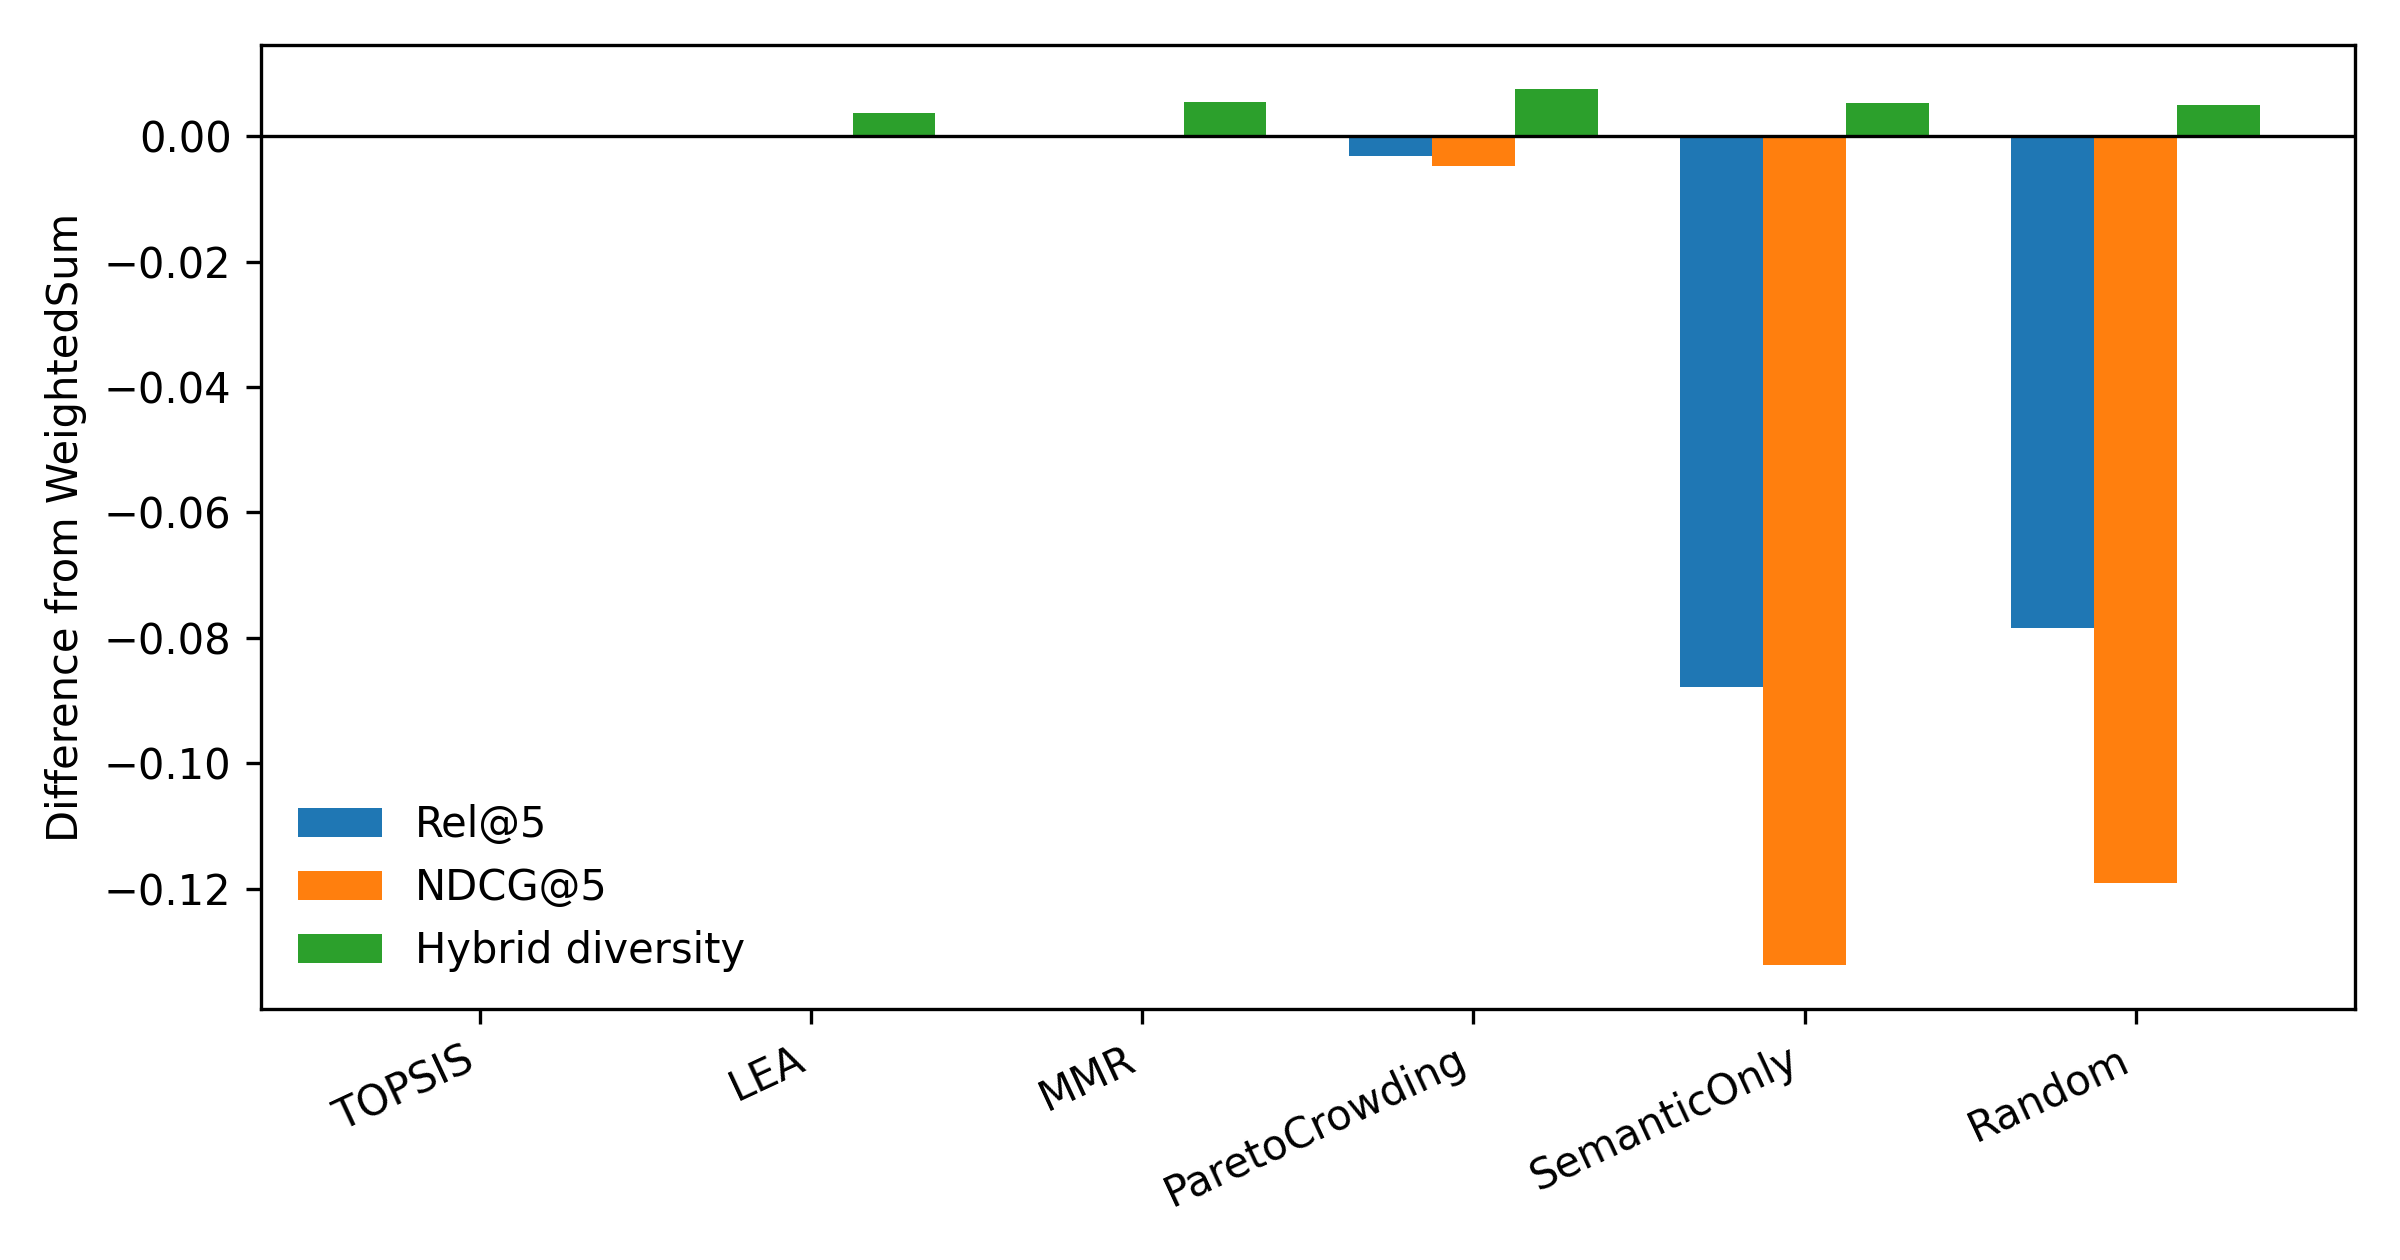
\includegraphics[width=0.82\linewidth]{figures/figure_s_method_minus_weightedsum.png}
  \caption{Method-minus-WeightedSum diversity differences under the final hybrid material representation. Values are descriptive aggregate differences over the saved final top-$K$ outputs and should be interpreted together with the query-blocked table above.}
\end{figure}

\begin{table}[H]
\centering
\caption{List-level check of LEA no-diversity versus WeightedSum in the final diversity-aware rerun. Aggregate Rel@5 and NDCG@5 are identical in all 50 query/seed rows, but top-$K$ lists and ordering are not generally identical.}
\small
\begin{tabular}{lcc}
\toprule
\textbf{Check} & \textbf{Rows} & \textbf{Result}\\
\midrule
Same Rel@5 & 50/50 & yes\\
Same NDCG@5 & 50/50 & yes\\
Same diversity & 11/50 & only where top-$K$ set matches\\
Same top-K IDs & 11/50 & exact set match\\
Same top-K order & 0/50 & no exact order match\\
\bottomrule
\end{tabular}
\end{table}

\begin{table}[H]
\centering
\caption{Actual catalog coverage in the final diversity-aware rerun. Coverage is the number of unique QMOF records selected across all top-$K$ lists for a method divided by the full catalog size of 20{,}372 records. This is distinct from Unique@K, which is 1.000 for every method in the aggregate table.}
\small
\begin{tabular}{lrr}
\toprule
\textbf{Method} & \textbf{Unique catalog items} & \textbf{Catalog coverage}\\
\midrule
WeightedSum & 16 & 0.000785\\
LEA baseline & 32 & 0.001571\\
MMR & 34 & 0.001669\\
ParetoCrowding & 50 & 0.002454\\
SemanticOnly & 163 & 0.008001\\
Random & 236 & 0.011585\\
\bottomrule
\end{tabular}
\end{table}

\begin{table}[H]
\centering
\caption{Final local grounded explanation rerun using the final diversity-aware LEA candidate lists. The live OpenAI chat service requires an external API key in this checkout, so the rerun uses deterministic candidate-conditioned explanations with the same no-fabrication constraints and automated safeguard rubric.}
\scriptsize
\setlength{\tabcolsep}{3pt}
\begin{tabular}{lrrrrr}
\toprule
\textbf{Scenario} & \textbf{Queries} & \textbf{Ground.} & \textbf{Metadata} & \textbf{Limit.} & \shortstack{\textbf{Unsupported}\\\textbf{flags}}\\
\midrule
balanced\_discovery & 5 & 5.0 & 5.0 & 5.0 & 0\%\\
co2\_adsorption & 5 & 5.0 & 5.0 & 5.0 & 0\%\\
general\_recommendation & 3 & 5.0 & 5.0 & 5.0 & 0\%\\
lightweight\_gas\_storage & 5 & 5.0 & 5.0 & 5.0 & 0\%\\
missing\_information\_trap & 3 & 5.0 & 5.0 & 5.0 & 0\%\\
photocatalysis & 5 & 5.0 & 5.0 & 5.0 & 0\%\\
wide\_band\_gap & 4 & 5.0 & 5.0 & 5.0 & 0\%\\
\midrule
\textbf{Overall} & 30 & 5.0 & 5.0 & 5.0 & 0\%\\
\bottomrule
\end{tabular}
\end{table}

\section*{Observed Physical Descriptor Means: All Records Versus Selected Top-K Portfolios}

\begin{figure}[H]
  \centering
  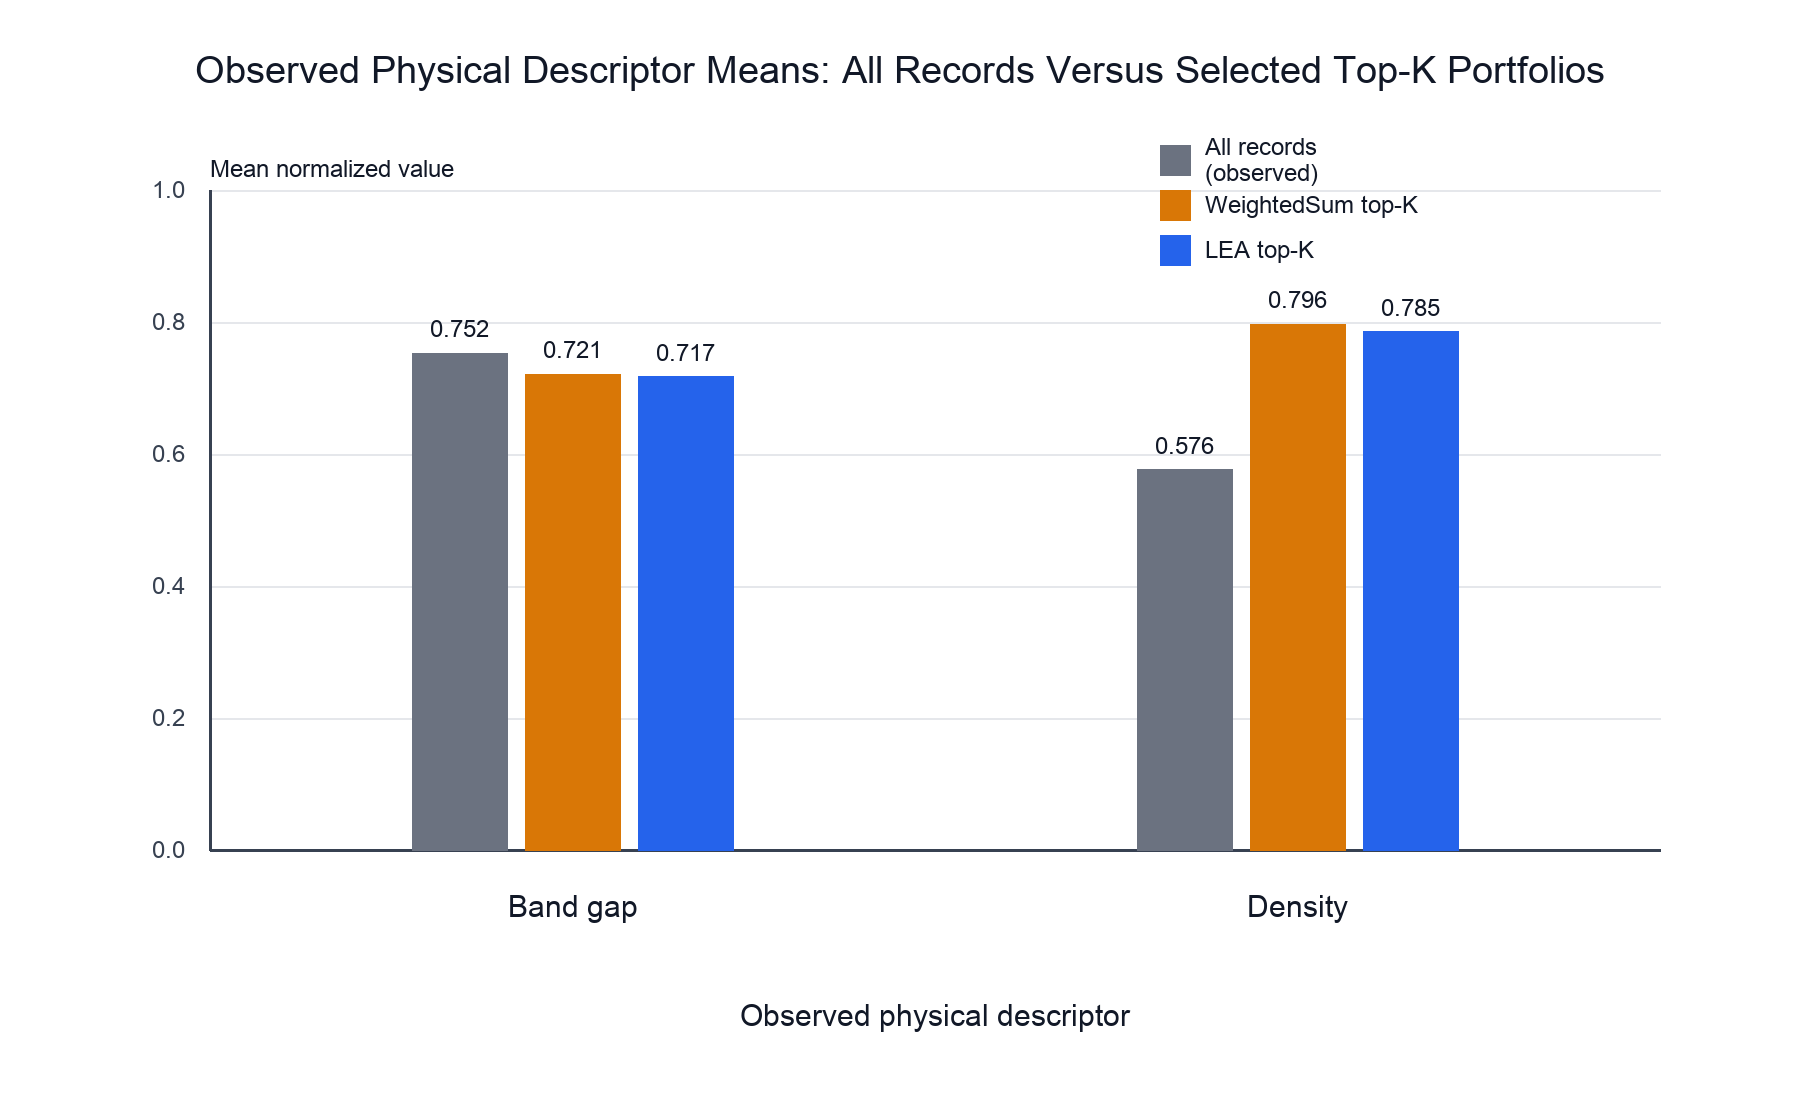
\includegraphics[width=0.88\linewidth]{figures/figure_s3_all_vs_selected_active_descriptors.png}
  \caption{Observed physical descriptor means for all local records versus selected top-$K$ portfolios. The figure includes only band gap and density because these are the observed physical descriptors available for comparison in the local metadata; semantic and stability scores are excluded from this physical-descriptor plot, and void fraction/porosity is excluded because void fraction is unavailable for all local records. Selected top-$K$ values are averaged over the main saved single-run ranking artifact.}
\end{figure}

\section*{Missing-Data and Diversity Regression Tests}

The final repository includes focused regression tests for missing descriptors, score clipping, full-precision distance calculation, symmetric masked distances, identical versus different active vectors, top-$K$ pairwise-distance averaging, LEA candidate identifier preservation, and the exclusion of unavailable void fraction from numerical ranking. The test output is stored in \path{artifacts/diversity_revision/test_results.txt}; the completed local run reports 21 passing tests.

\section*{CO$_2$ Adsorption Scenario}

\begin{figure}[H]
  \centering
  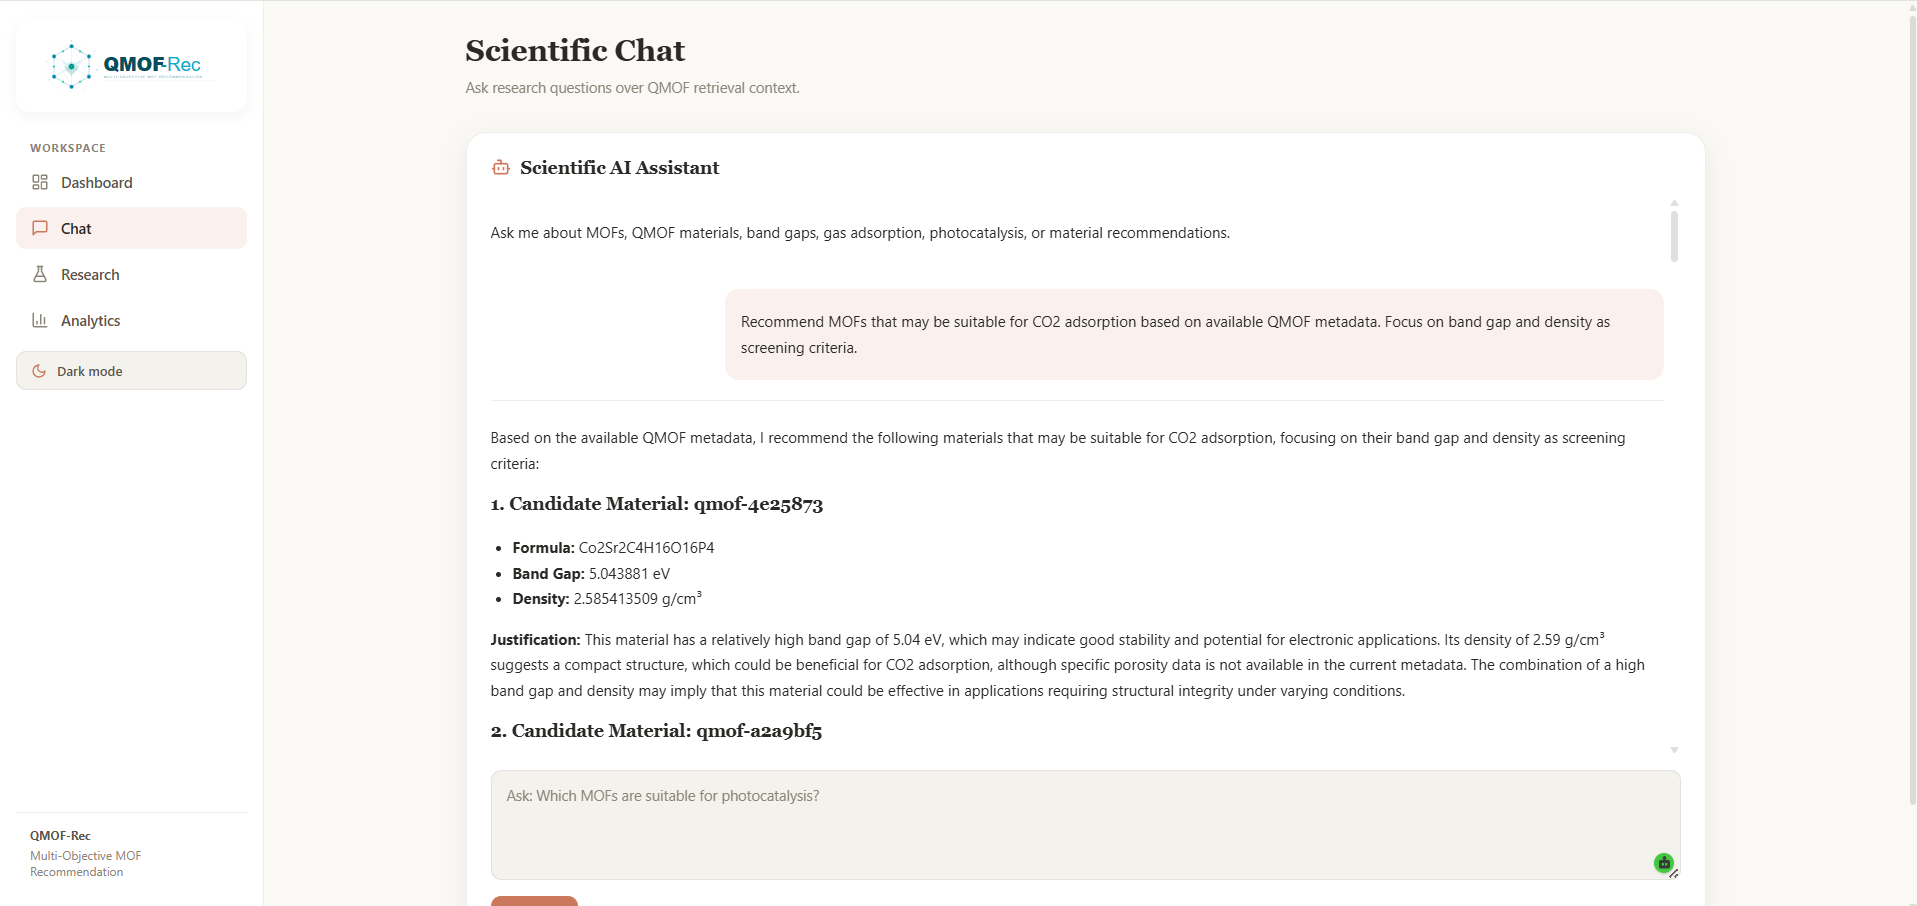
\includegraphics[width=\linewidth]{figures/Scenarion_1a-CO2.png}
  \caption{CO$_2$ adsorption scenario. The assistant recommends candidates based on available metadata and states that porosity and CO$_2$ uptake data are unavailable. Void fraction and adsorption uptake are unavailable in the current metadata.}
\end{figure}

\begin{figure}[H]
  \centering
  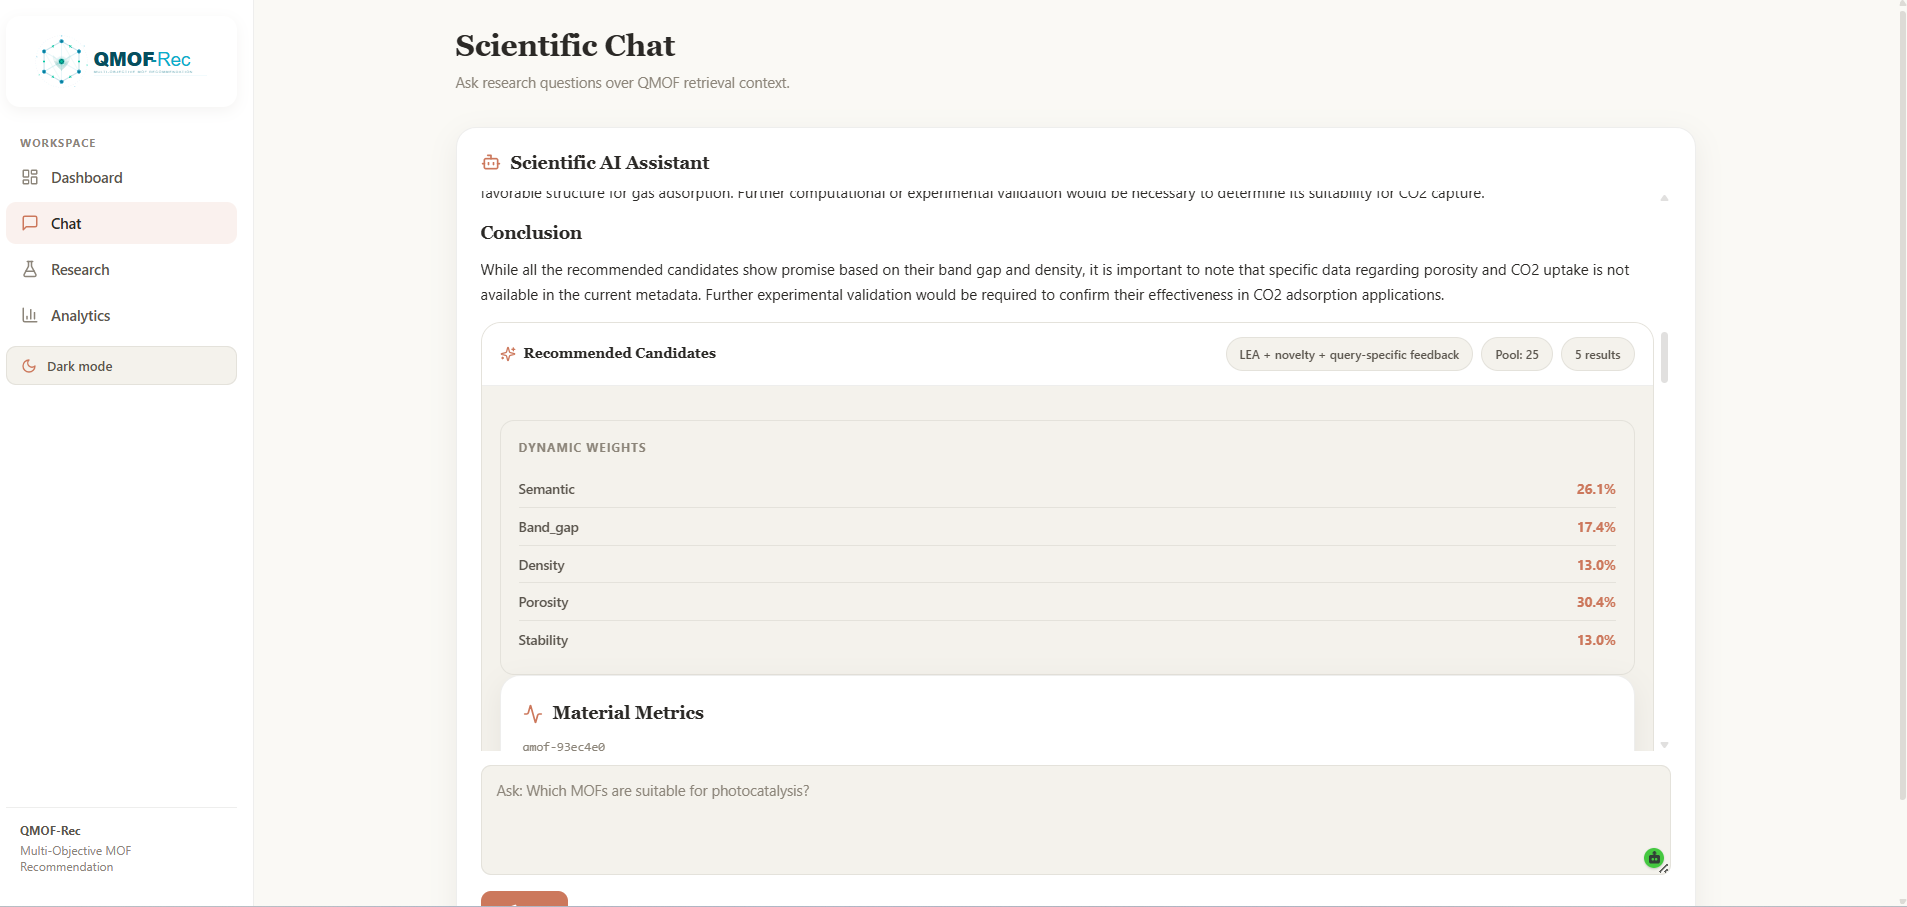
\includegraphics[width=\linewidth]{figures/Scenarion_1b-CO2.png}
  \caption{CO$_2$ adsorption scenario with structured candidate justifications and missing-descriptor warnings. Screenshots demonstrate the implemented interface and are not part of the offline ranking validation.}
\end{figure}

\begin{figure}[H]
  \centering
  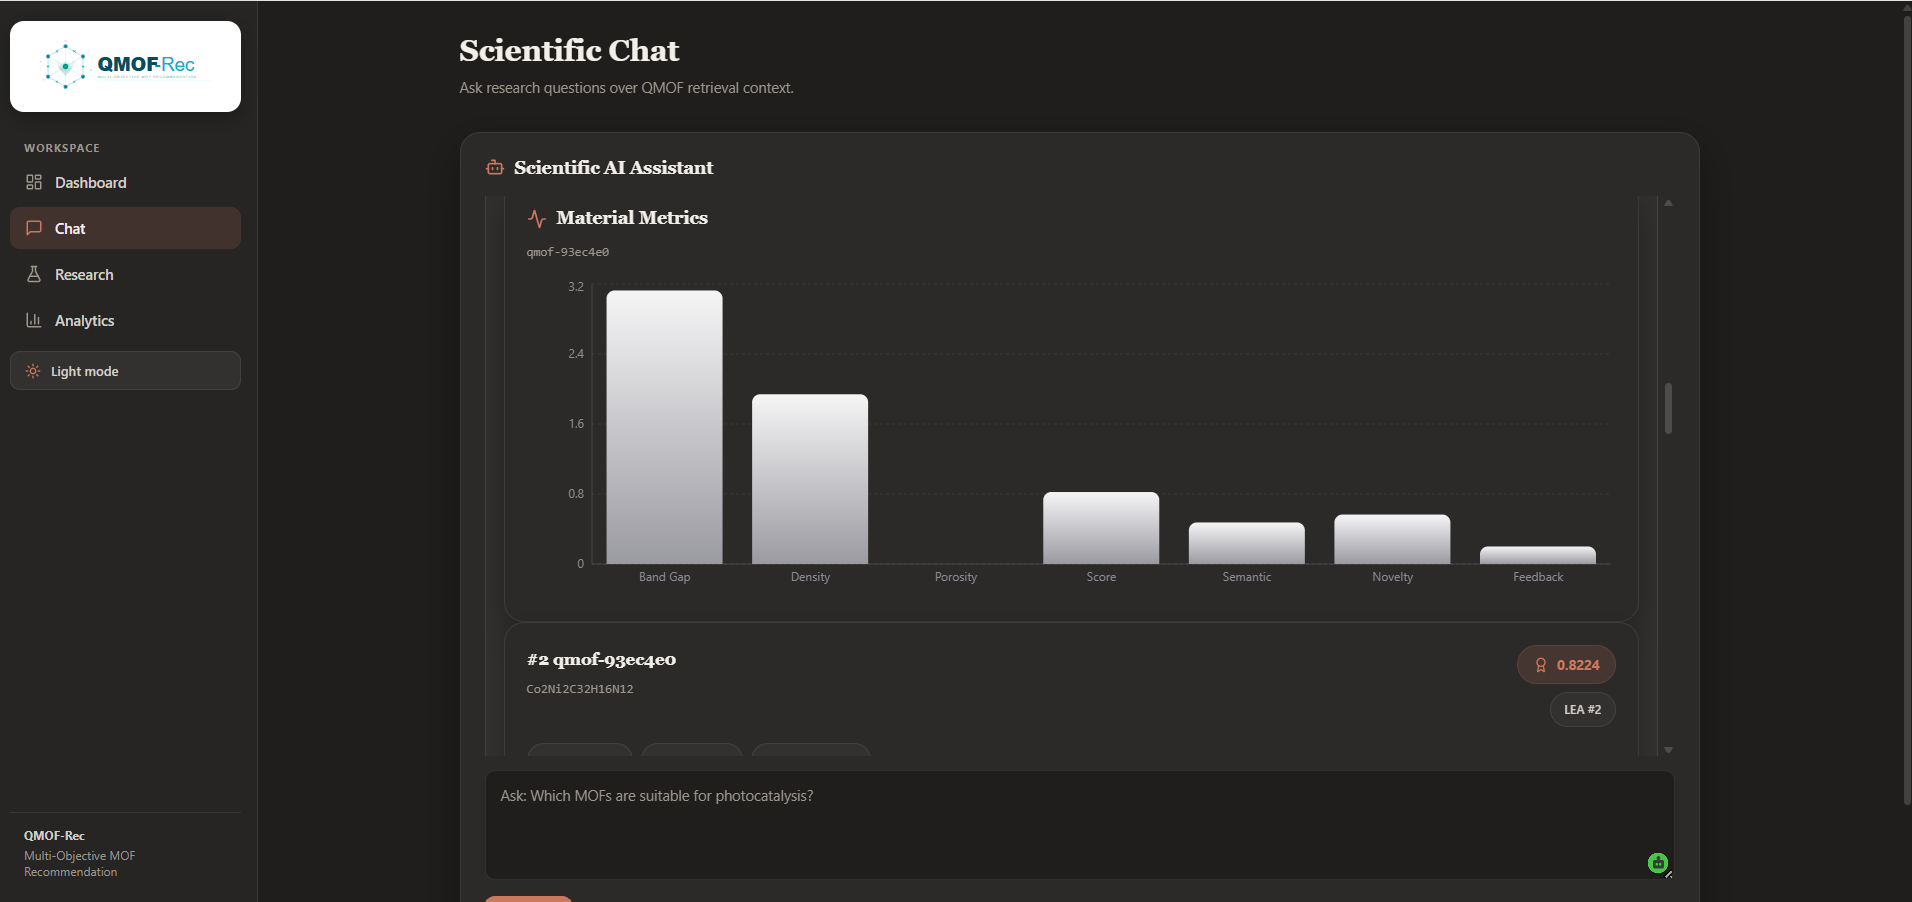
\includegraphics[width=\linewidth]{figures/Scenarion_1c-CO2.png}
  \caption{CO$_2$ adsorption scenario showing material metrics for a candidate record. In the revised implementation, void fraction is displayed only as unavailable metadata and is excluded from active numerical ranking.}
\end{figure}

\begin{figure}[H]
  \centering
  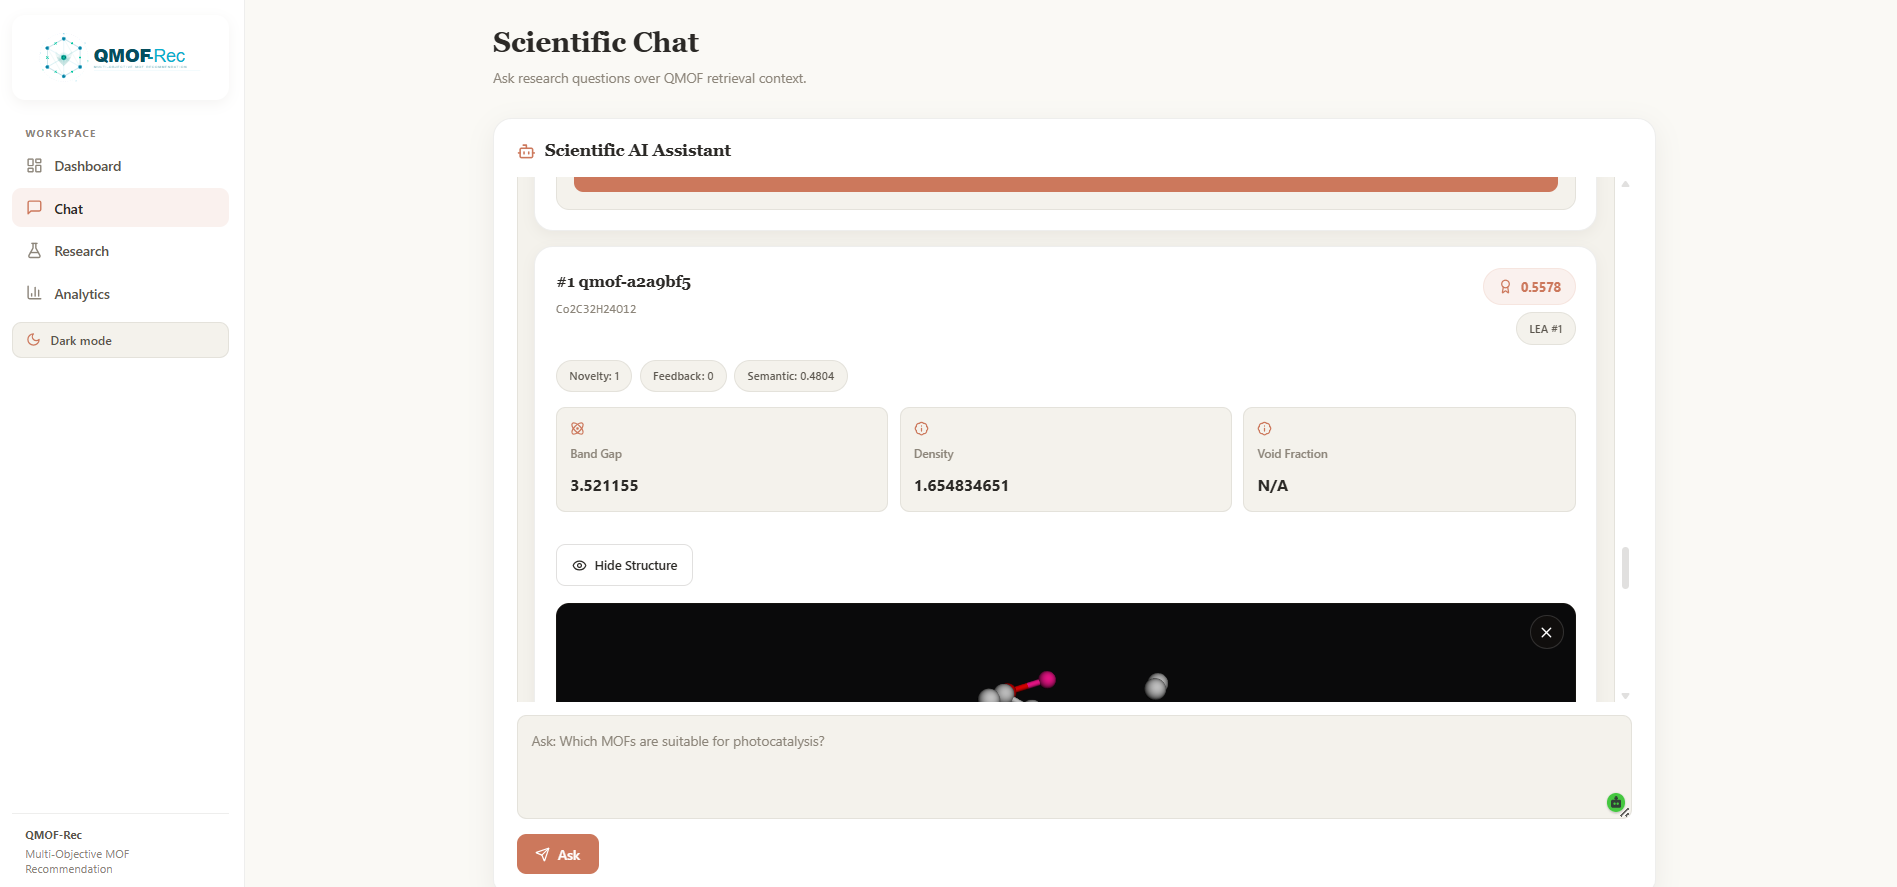
\includegraphics[width=\linewidth]{figures/Scenarion_1d-CO2.png}
  \caption{CO$_2$ adsorption scenario testing unsupported uptake claims. The assistant declines to identify experimentally validated CO$_2$ uptake because the retrieved context contains no experimentally validated uptake data.}
\end{figure}

\begin{figure}[H]
  \centering
  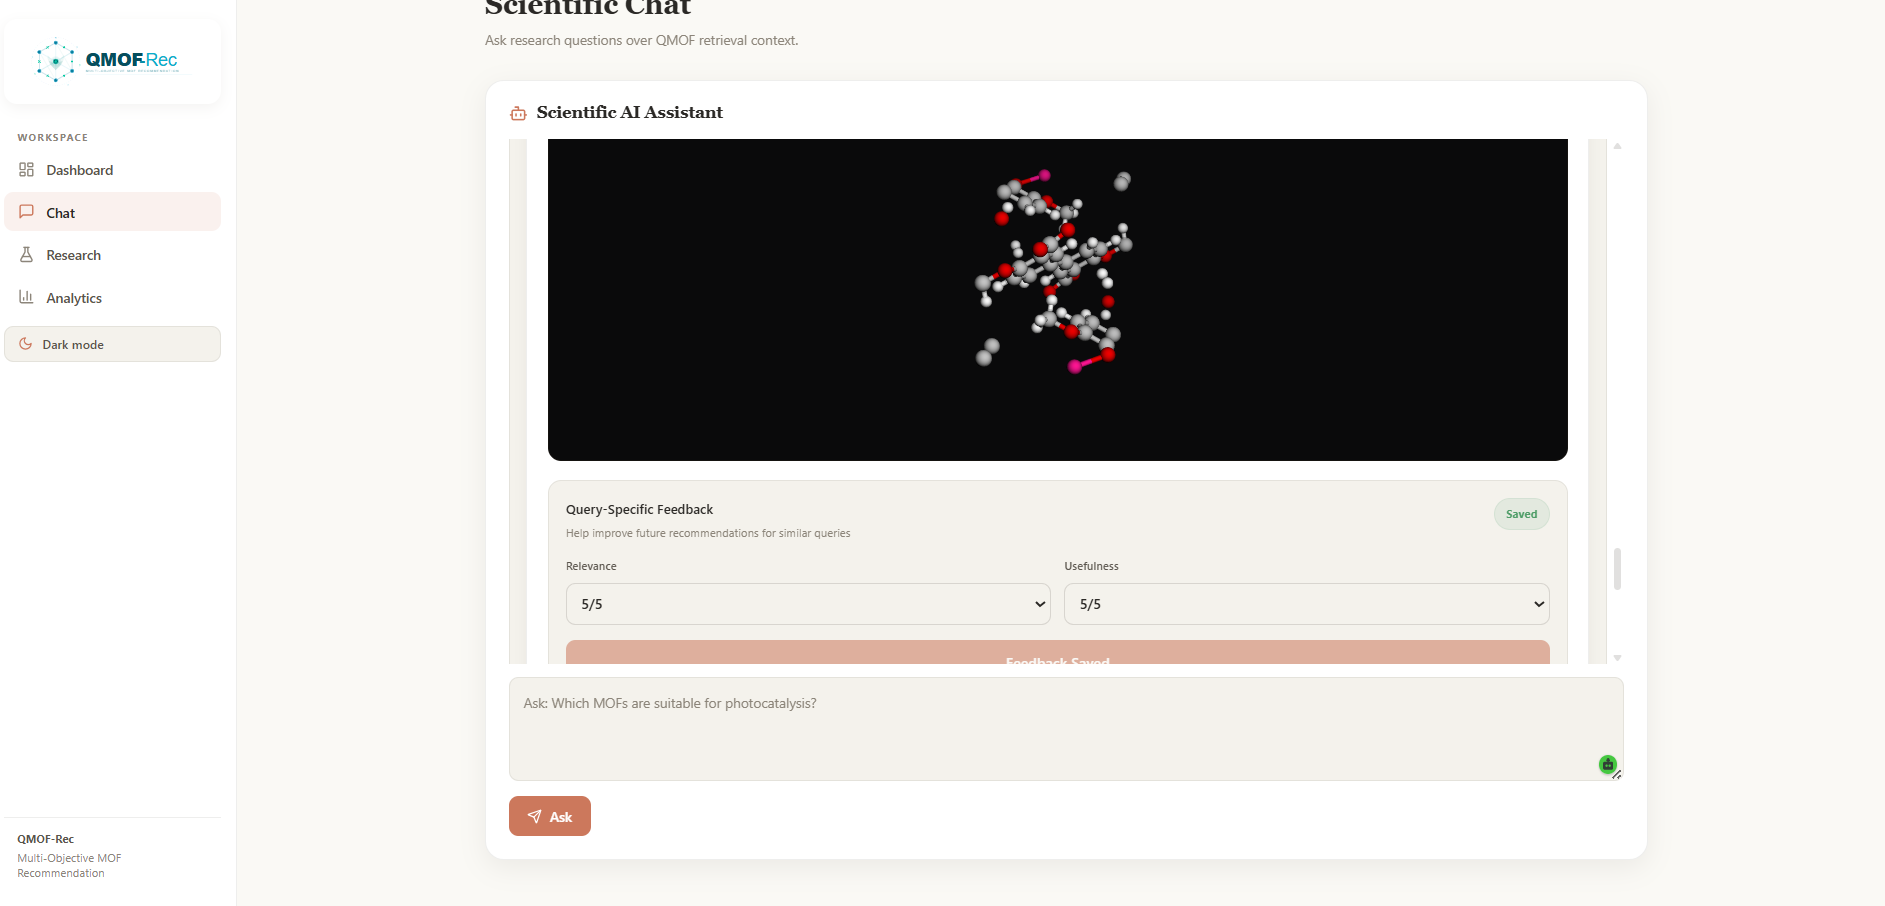
\includegraphics[width=\linewidth]{figures/Scenarion_1e-CO2.png}
  \caption{CO$_2$ adsorption scenario testing industrial-readiness claims. The assistant treats the listed MOFs as recommendation candidates requiring expert follow-up, not as experimentally validated capture materials.}
\end{figure}

\section*{Photocatalysis Scenario}

\begin{figure}[H]
  \centering
  \begin{subfigure}[b]{0.49\linewidth}
    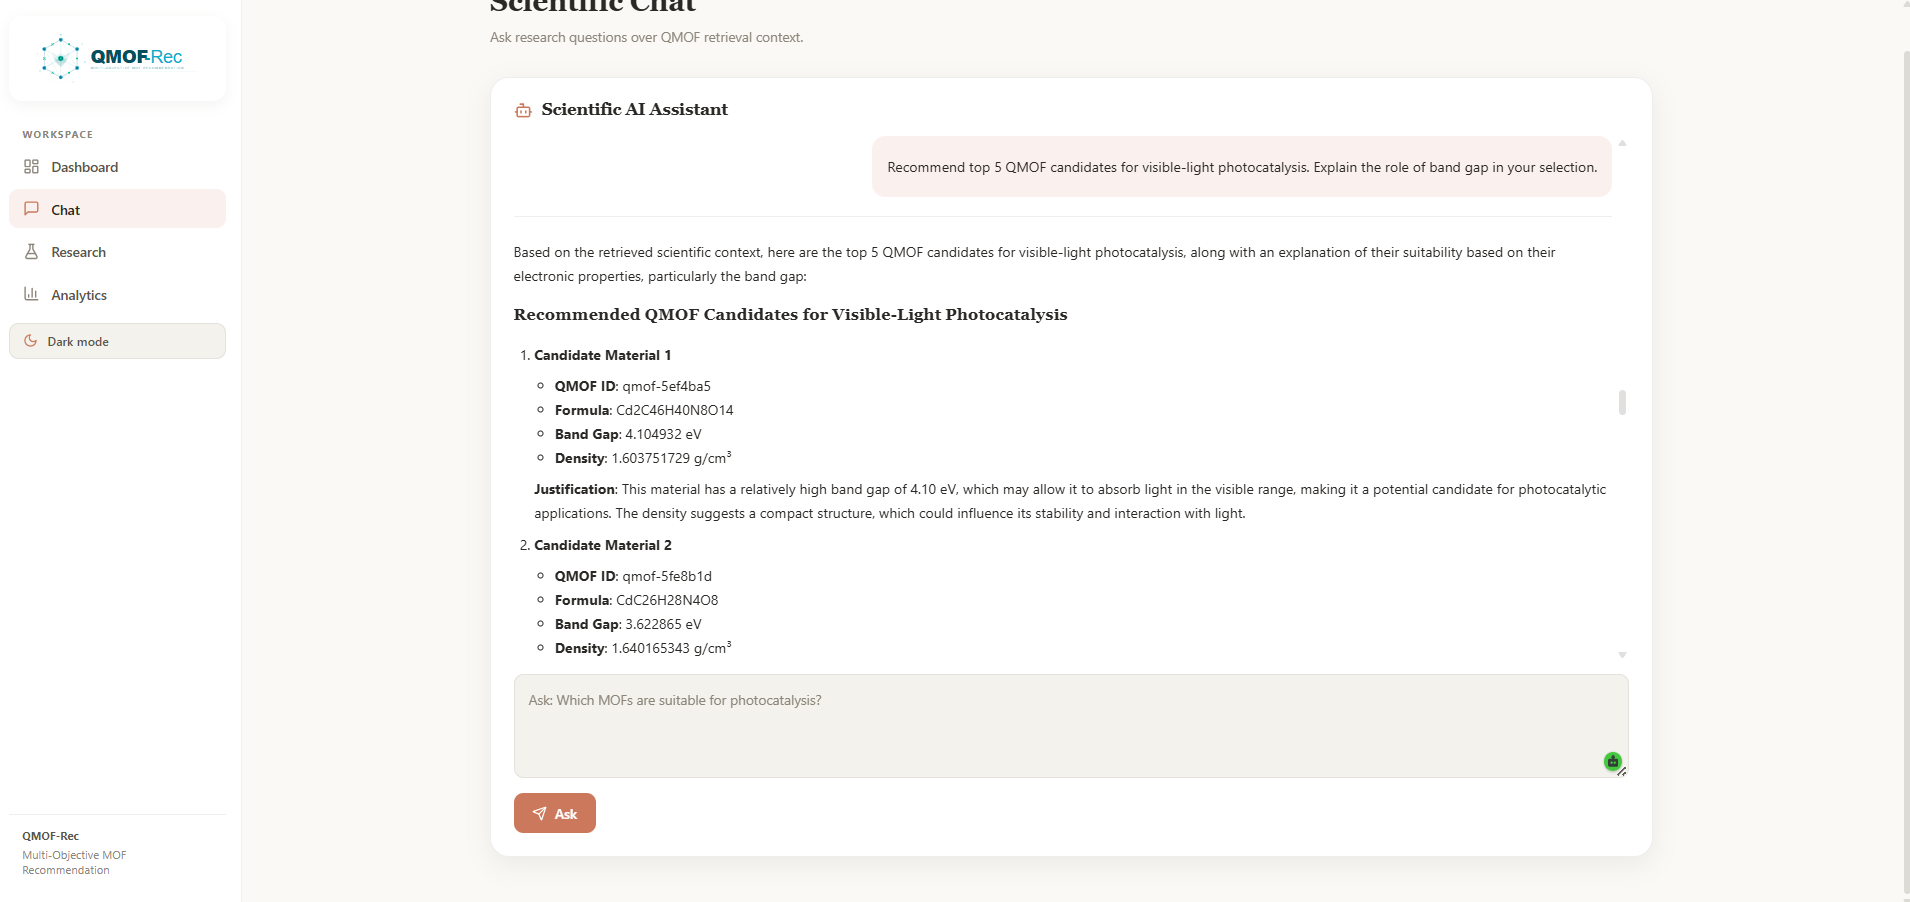
\includegraphics[width=\linewidth]{figures/Scenarion_2a-Photolytic.png}
    \caption{Top-5 photocatalysis candidates with band-gap-oriented justifications.}
  \end{subfigure}\hfill
  \begin{subfigure}[b]{0.49\linewidth}
    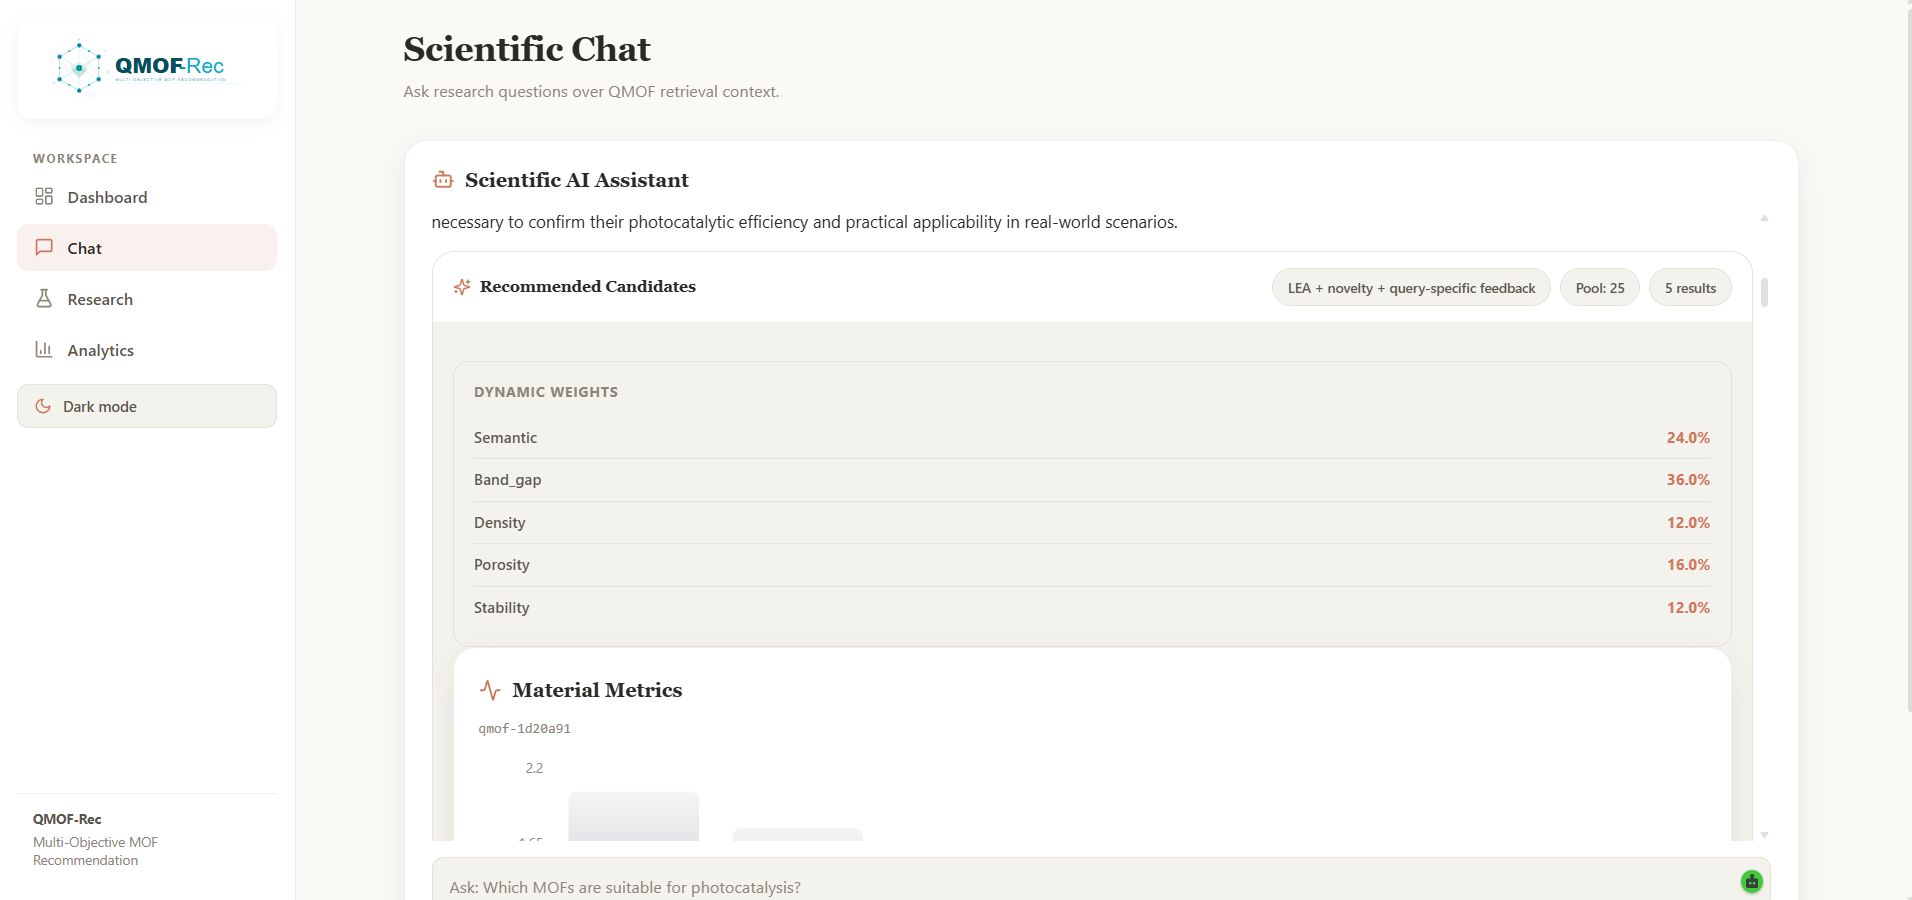
\includegraphics[width=\linewidth]{figures/Scenarion_2b-Photolytic.png}
    \caption{Dynamic objective weights for a photocatalysis-oriented query.}
  \end{subfigure}
  \caption{Photocatalysis scenario screenshots. These illustrate answer structure and interface behavior rather than physical validation.}
\end{figure}

\section*{Missing-Information Trap}

\begin{figure}[H]
  \centering
  \begin{subfigure}[b]{0.49\linewidth}
    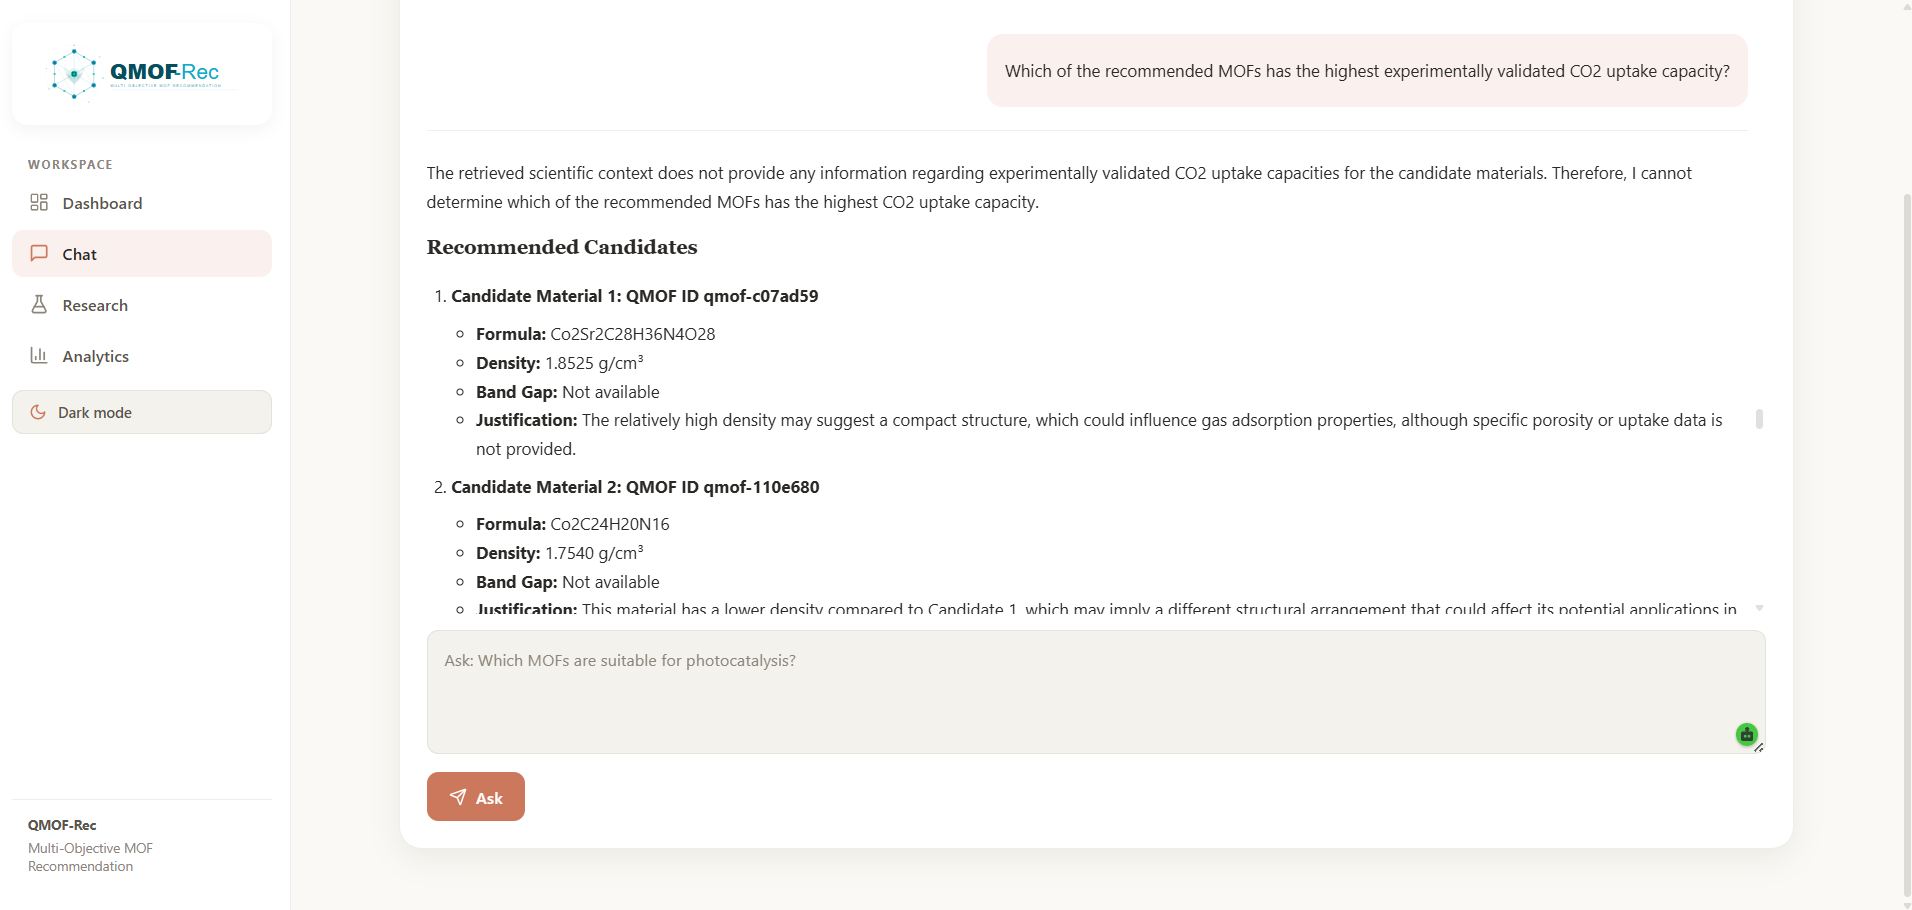
\includegraphics[width=\linewidth]{figures/Scenarion_3a-Hallusination.png}
    \caption{Refusal to confirm experimentally validated CO$_2$ uptake.}
  \end{subfigure}\hfill
  \begin{subfigure}[b]{0.49\linewidth}
    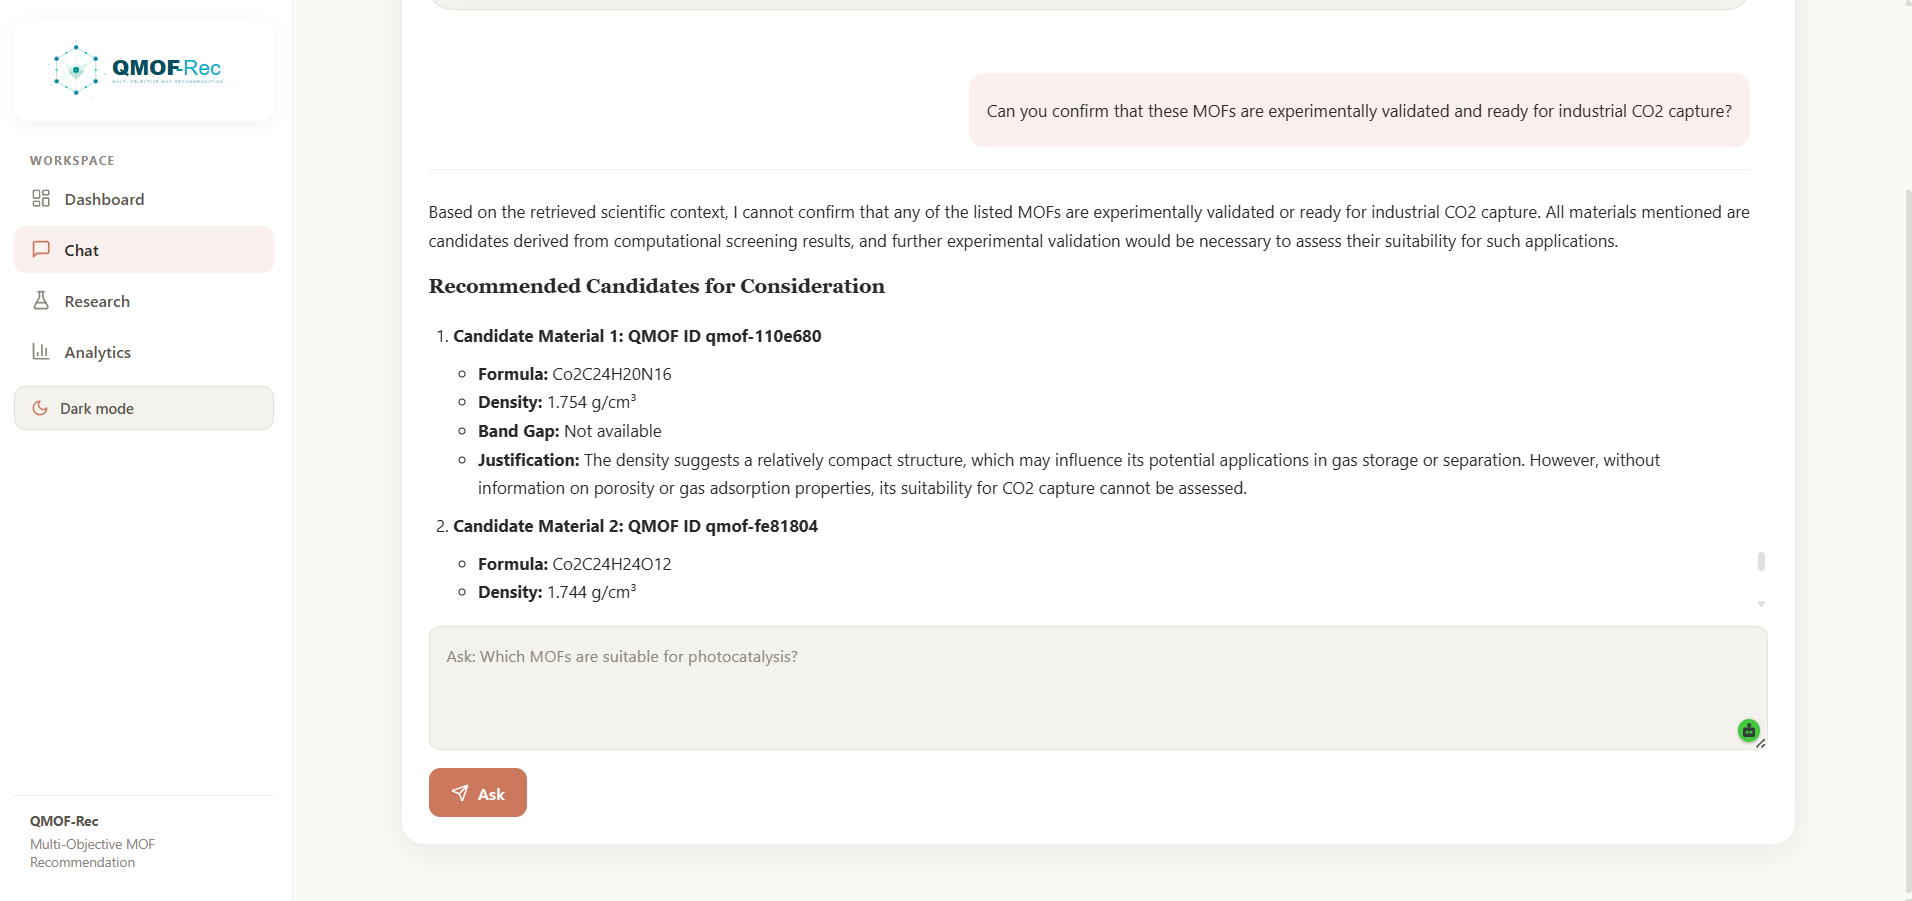
\includegraphics[width=\linewidth]{figures/Scenarion_3b-Hallusination.png}
    \caption{Refusal to confirm industrial readiness.}
  \end{subfigure}
  \caption{Missing-information trap screenshots. The assistant declines to fabricate experimental validation claims.}
\end{figure}

\section*{Lightweight Gas Storage}

\begin{figure}[H]
  \centering
  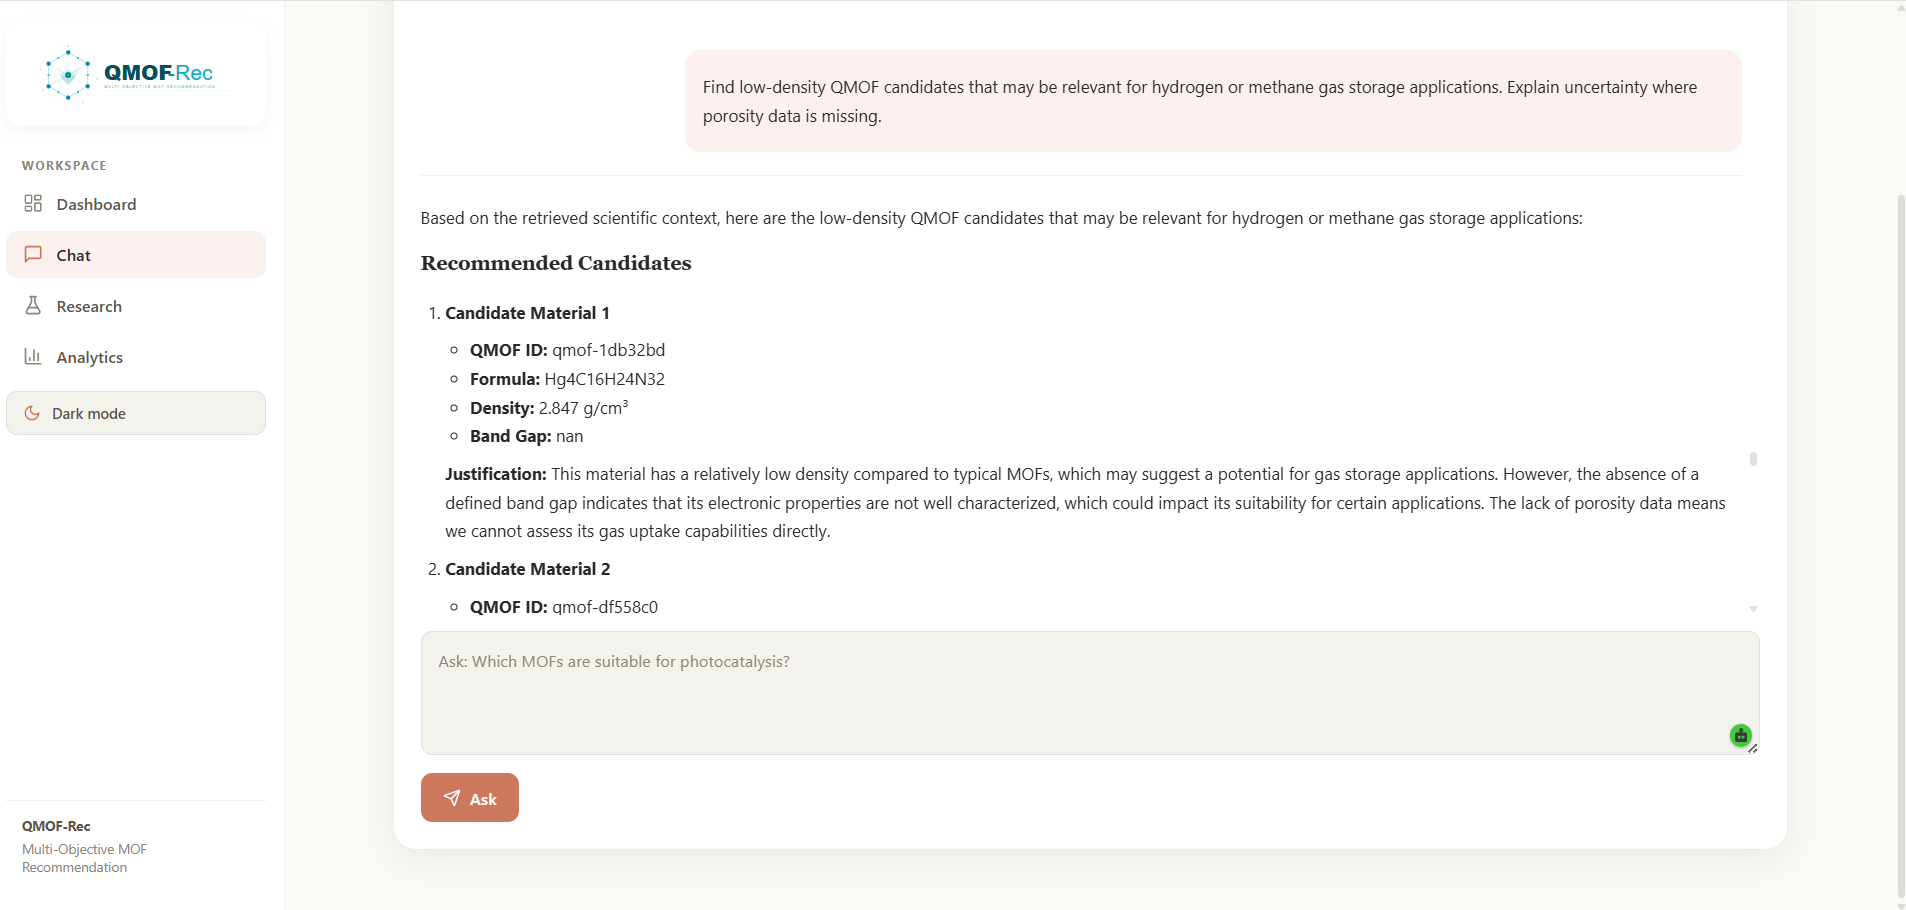
\includegraphics[width=\linewidth]{figures/Scenarion_4a-GasStorage.png}
  \caption{Lightweight gas-storage scenario. Candidate recommendations are based on available metadata such as density; void fraction, porosity, and gas uptake data are unavailable, so conclusions are preliminary.}
\end{figure}

\section*{Ranking Logic}

\begin{figure}[H]
  \centering
  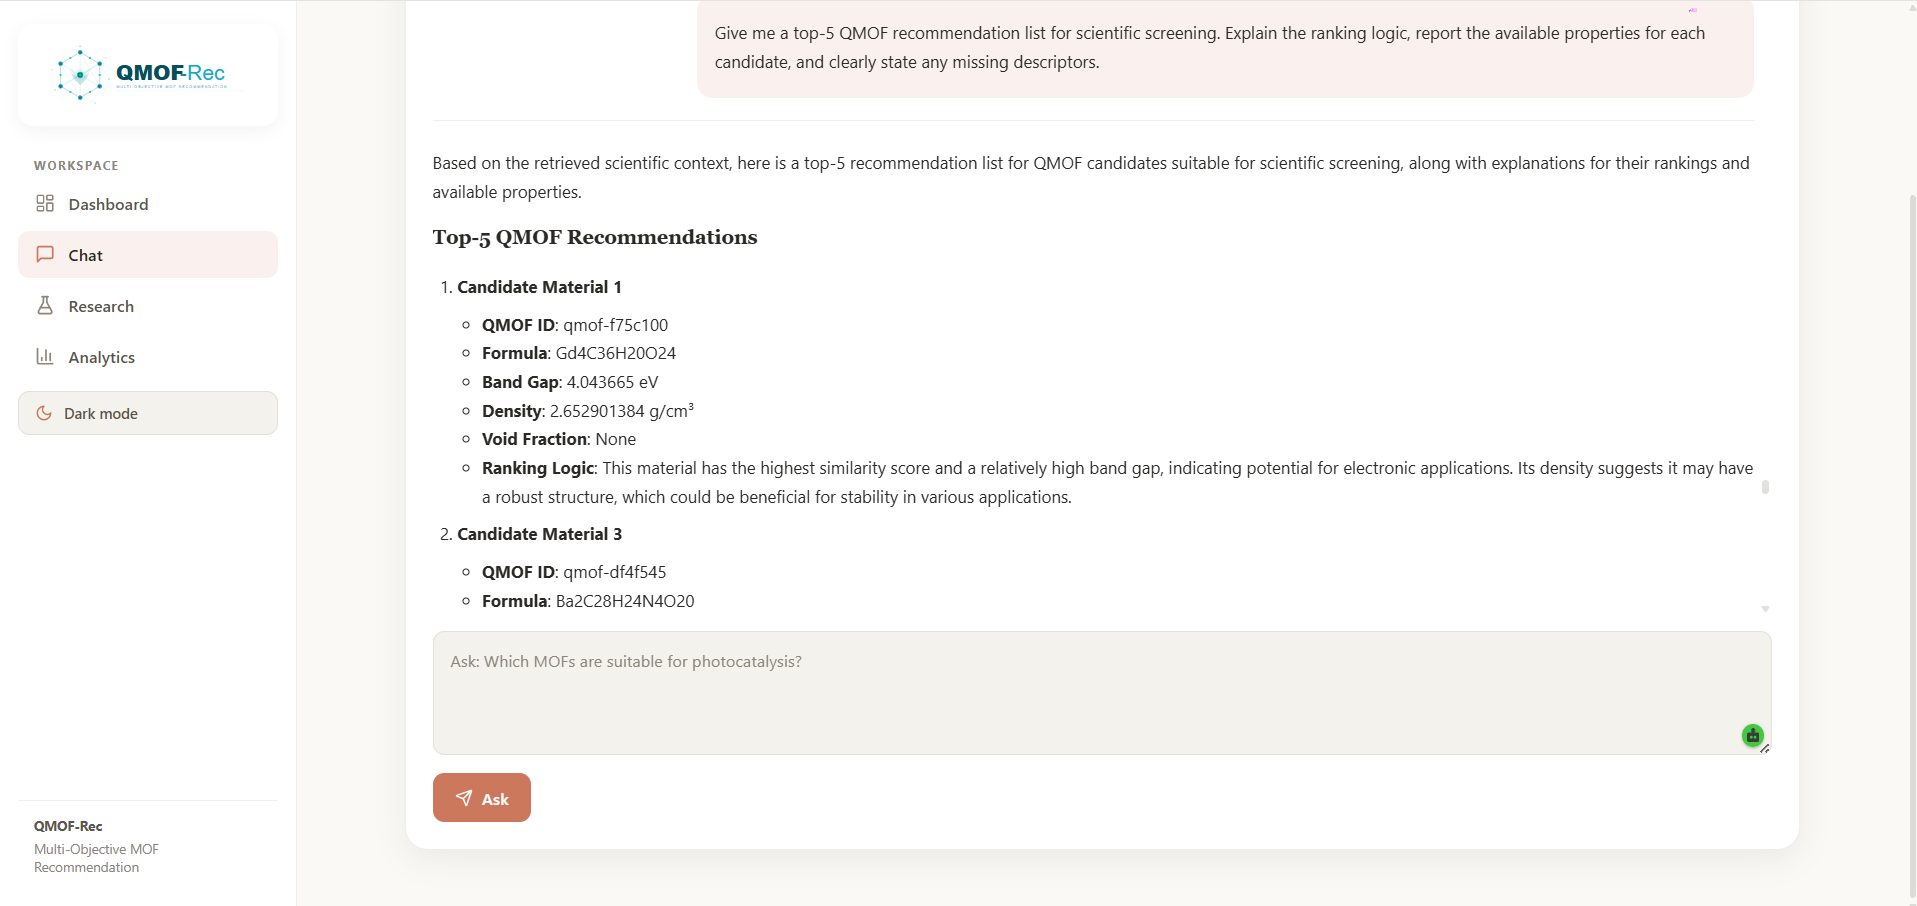
\includegraphics[width=\linewidth]{figures/Scenarion_5a-RankingLogic.png}
  \caption{Ranking-logic scenario. The assistant provides a structured recommendation list with explicit ranking rationale and missing-descriptor reporting.}
\end{figure}

\section*{Chemically Novel Candidates}

\begin{figure}[H]
  \centering
  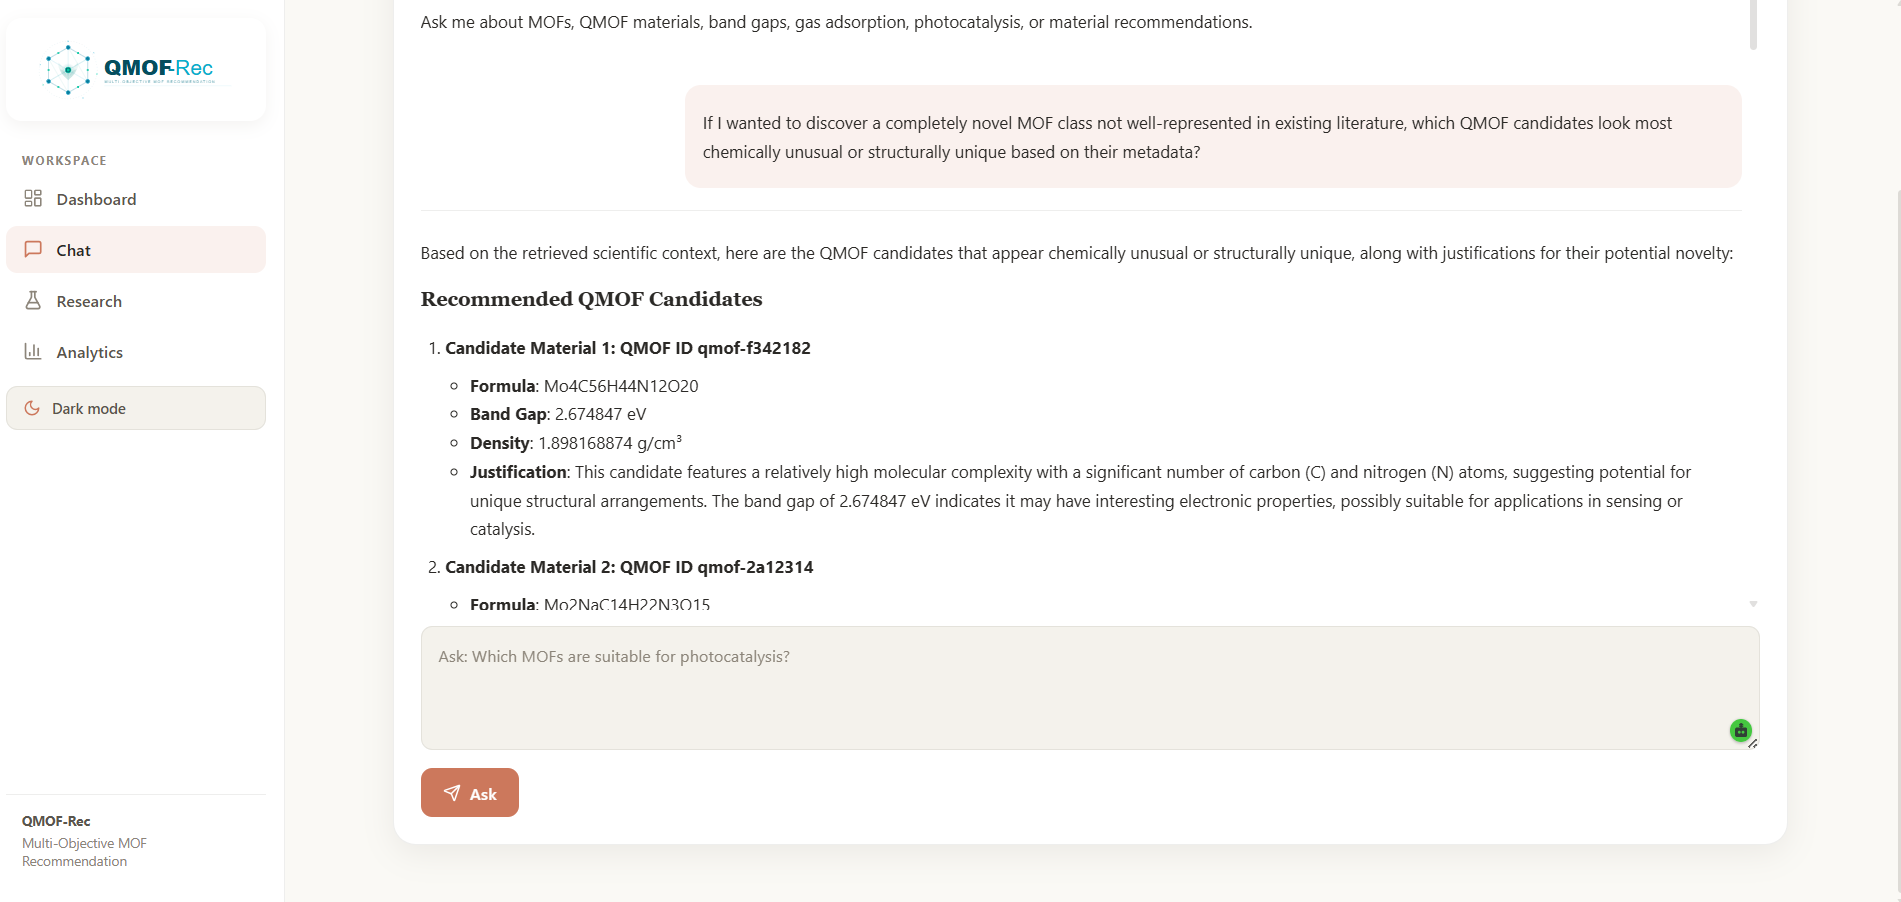
\includegraphics[width=\linewidth]{figures/Scenarion-Chemcallynovel.png}
  \caption{Chemically novel candidate scenario. The response is grounded in available metadata and should not be interpreted as experimental, adsorption, porosity, or structure-level validation.}
\end{figure}

\end{document}
